% DO NOT CHANGE THIS SEGMENT
% vvvvvvvvvvvvvvvvvvvvvvvvvvvvvvvvvvvvvvvvv
\documentclass[10pt,twocolumn,twoside,a4paper]{article}
% * <rbatzing@gmail.com> 2017-12-11T08:03:48.862Z:
%
\usepackage{mathspec}
\usepackage{polyglossia}
%\setdefaultlanguage[numerals=thai]{thai}
\setdefaultlanguage{thai}
\setotherlanguage{english}
\setmainfont{FreeSerif}
\setsansfont{FreeSerif}
\setmonofont[Scale=1.25,Numbers={Monospaced,Lining},Color=003366]{FreeSerif}
\newfontfamily{\thaifonttt}[Scale=1.25,Numbers={Monospaced,Lining},Color=003366]{FreeSerif}
\setmathsfont(Digits,Latin,Greek){FreeSerif}
\newfontfamily{\thaifont}[Script=Thai,Scale=1.2]{FreeSerif}
\XeTeXlinebreaklocale "th"
\hyphenation{sledge-ham-mer}
%%%%
\usepackage{url}
\usepackage{hyperref}
\usepackage{authblk}
\usepackage{graphicx}
\usepackage{algorithm}
\usepackage{algorithmicx}
\usepackage{algpseudocode}
\usepackage{array}
\usepackage{stfloats}
\usepackage{flushend}
\usepackage{ntheorem}
\usepackage{listings}
\usepackage{datetime}
\newtheorem{hyp}{สมมติฐานที่}
\gdef\gb{\hfil\penalty -1000}
\usepackage{listings}
\usepackage{titling}
\usepackage[usenames,dvipsnames,svgnames]{xcolor}
%^^^^^^^^^^^^^^^^^^^^^^^^^^^^^^^^^^^^
%%%%%%%%%%%%%%%%%%%%%%%%%%%%%%
% Title and Author
% Change for each document
\title{โครงสร้างเอกสารรายงานการวิจัย%
\thanks{This manuscript has been developed as a template for students use for technical reports. Last revised: 11~December 2017}\\
A Starter-File for Research Reports}
\author{อ.~ดร.~โรเบิร์ท~แบทซิงเงอร์\thanks{Dr. Robert P. Batzinger, Computer Science Instructor Emeritus, Payap University; 
email: \texttt{robert$\_$b@payap.ac.th}}\and
อ.~นิภาภรณ์~เอื้อตรงจิตต์\thanks{Ms. Nipaporn Euathrongchit, Computer Science Instructor, Payap University; 
email: \texttt{gengjang@payap.ac.th}}}%
\date{สาขาวิชาวิทยาการคอมพิวเตอร์ คณะวิทยาศาสตร์\\
    มหาวิทยาลัยพายัพ จังหวัดเชียงใหม่ 50000\\
    ประเทศไทย}
%%vvvvvvvvvvvvvvvvvvvvvvvvvvvvvvvvvvvvvvvv
% Document settings DO NOT CHANGE
\setlength{\droptitle}{-1.2in}% First page to the top
\providecommand{\keywords}[1]{\noindent\textbf{\textit{Keywords---}} #1}
\bibliographystyle{IEEEtran}% IEEE reference style used
\pagestyle{myheadings}
\markboth{\hfill\thetitle}{File: \jobname:\ Compiled: \today \currenttime\hfill}
\linespread{1.5}% linespace for Thai docs
\setlength{\columnsep}{1cm}
\setlength{\columnwidth}{8cm}
\newcounter{cf}
\newfloat{code}{h}{cf}
\floatname{code}{ตัวอย่างโค้ดที่}
\floatname{algorithm}{ขั้นตอนวิธีที่}
\floatstyle{plaintop}
\restylefloat{code}
\restylefloat{table}
\floatstyle{plain}
\restylefloat{figure}
\lstset{firstline=1,numbers=left,
numbersep=7pt,frame=shadowbox,
keywordstyle=\color{DarkGreen},
basicstyle=\footnotesize,
xleftmargin=20pt,xrightmargin=10pt,
rulesepcolor=\color{DarkBlue},
backgroundcolor=\color{LightYellow}}
%%^^^^^^^^^^^^^^^^^^^^^^^^^^^^^^^^^^^^
%%%%%%%%%%%
\begin{document}
\thispagestyle{empty}%
\maketitle

\begin{abstract}
This paper demonstrates the format and common components of IEEE papers developed using the standard \LaTeXe\ template file. The purpose of this document is to provide a starting point for student research reports. This starter document has been designed to support the Thai language without the need for special commands to switch languages. Students can use this document as a to submit their work in Thai or English.will s learning to develop publishable reports of their findings.
\end{abstract}

\bigskip
\keywords{\LaTeX, research paper, student template, Thai document support, เอกสารรายงานการวิจัย}

\section{บทนำ}
This demo file is intended to serve as a ``starter file''
for IEEE/ACM journal papers produced under \LaTeX\ using the double-column/double-sided page article format. The paper was developed using a web browser and a free account at \url{http://www.overleaf.com} reducing the need to download and install \LaTeXe\ on a local computer. 

The class logo is seen as a floating illustration in Figure~\ref{fig_classlogo}.

\begin{figure}[htb]
\centering
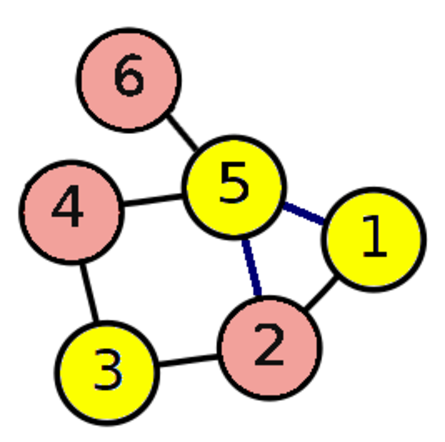
\includegraphics[width=2in]{img/classlogo.pdf}
\caption{The class logo}
\label{fig_classlogo}
\end{figure}

In general the Introduction Section needs answer the following questions:

\begin{itemize}
\item What is the context of this research and why is it important? \texttt{\ref{background}~Background}
\item What has already been published about this area?  \texttt{\ref{litreview}~Literature Review}
\item What do you expect to be able to show with this research? \texttt{\ref{purpose}~Purpose and Research Objectives}
\item What outcomes do you expect?
\texttt{\ref{expectation}~Expected outcomes}
\end{itemize}

Summary of the research question. 
Figure~\ref{fig_doublecolumn} is an example of a double column floating figure that extends to the width of the page.

\begin{figure*}[!t]
\centering
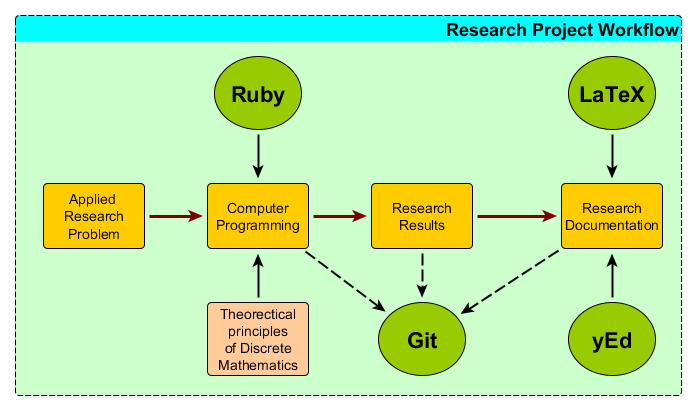
\includegraphics[width=\textwidth,height=3in]{img/researchprojectWork.png}%
\caption{Typical project work flow.}
\label{fig_doublecolumn}
\end{figure*}

\subsection{หลักการและเหตุผล}
\label{background}
Overview and background text to describe why this will be an interesting paper.

\subsection{การทบทวนวรรณกรรม}
\label{litreview}
Summary of published papers and references on this subject complete with citation.
The class textbook\cite{Levin:2017} is a good starting point.


\begin{table}[htb]
\caption{A list of textbooks used for the course}
\label{textbookList}
\medskip
\centering
\small
\begin{tabular}{p{1.25in}rc}
\textbf{Author} & \textbf{Pages} & \textbf{Doc Type}\\
Code School\cite{CodeSchool:2013} & 20 & Ruby\\
Kopka\cite{Kopka:2003} & 559 & \LaTeX \\
Kwong\cite{Kwong:2015} & 307 & DisMath\\
Levin\cite{Levin:2017} & 345 & DisMath\\
Oetiker et als\cite{Oetiker:1996} & 63 & \LaTeX\\
Pine\cite{Pine:2014} & 216 & Ruby \\
Stein et als\cite{Stein:2011} & 526 & DisMath\\
Thomas\cite{Thomas:2013} & 863 & Ruby \\
สมชาย\gb ประสิทธิ์จูตระกูล\cite{Somchai:2011} & 339  & DisMath\\
\end{tabular}
\end{table}

\subsection{ปัญหาที่พบ}
\label{purpose}


It is also good to include relevant mathematic formula. This is relatively easy to do as shown by the Taylor series for approximating the value of $e^x$ given in Equation~\ref{taylorseries}.

\begin{equation}
\label{taylorseries}
e^x = {x^0\over 0!} + {x^1\over 1!} + {x^2\over 2!} +{x^3\over 3!} + ...= \sum^\infty_{n=0}\ {x^n\over n!}
\end{equation}

One can include flowing text as well as seen in Table \ref{Proverbs}

\begin{table}[htb]
\caption{Thai Proverbs}
\label{Proverbs}
\medskip
\begin{tabular}{p{0.4\columnwidth} p{0.5\columnwidth}}
\hfil\textbf{ภาษาไทย} & \hfil\textbf{English}\\
งมเข็มในมหาสมุทร & Look for a needle in a haystack.\\
ขี่ช้างจับตั๊กแตน & Use a sledgeham\-mer to crack a nut.\\
น้ำตาลใกล้มด & Bees around honey \\
นกน้อยทำรังแต่พอตัว & Living within your means\\
แมวไม่อยู่ หนูร่าเริง & When the cat’s away the mice will play.\\
\end{tabular}
\end{table}


\subsection{ผลที่คาดว่าจะได้}
\label{expectation}

Clearly state the postulated or expected results of this work. Provide a listing of the hypothetical outcomes.

\begin{hyp}
The better the answer, the higher the score.
\end{hyp}

\begin{hyp}
The higher the score the better the grade
\end{hyp}

\section{ระเบียบวิธี}
\label{methodology}
Describe the programming environment and the approach used to collect data to address the research question being addressed.
Many parameters can be listed in a simple table as shown in  Table \ref{environment}

\begin{table}
\caption{Programming environment}
\label{environment}
\begin{tabular}{lc}
\textbf{Parameter} & \textbf{Value}\\
CPU & Z80, 1 MHz\\
RAM Memory & 16 K\\
Ext Memory & 1 MB\\
Programming language & C \\
Communication& Bluetooth \\
\end{tabular}
\end{table}

A simple flowchart like that in Figure \ref{fig_flowchart} is a great way to illustrate the critical logic.

\begin{figure}[htb]
\centering
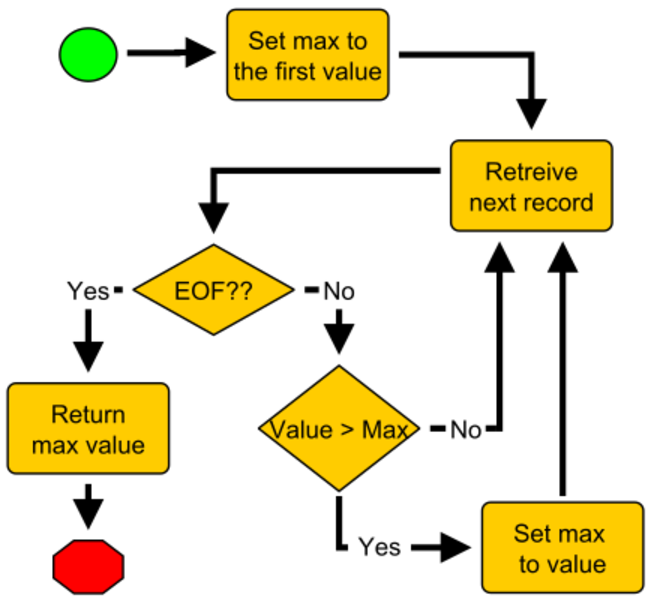
\includegraphics[width=\columnwidth]{img/flowchart.pdf}
\caption{Logic of the Max() Function}
\label{fig_flowchart}
\end{figure}

\section{ผลการวิจัย}
\label{results}

Provide tables and graphs that summary of the information collected. Figure \ref{fig_experiment}
is a scatterplot of experimental data. 

\begin{figure}[htb]
\centering
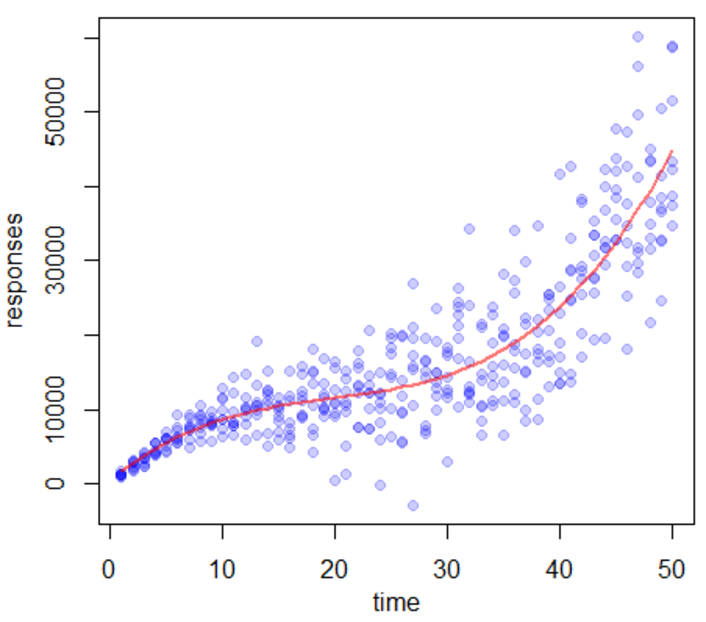
\includegraphics[width=\columnwidth,
height=\columnwidth]{img/experiment.pdf}
\caption{Experimental data}
\label{fig_experiment}
\end{figure}


Floating figures will be placed in the next appropriate place. For example, Figure \ref{fig_histogram} is a histogram created in R.

\begin{figure}[htb]
\centering
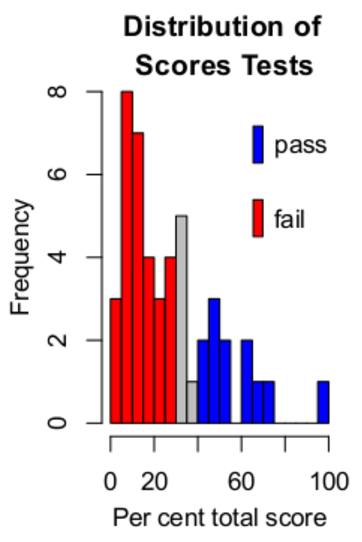
\includegraphics[width=\columnwidth,height=\columnwidth]{img/Rplot.pdf}
\caption{Freshmen Math Grades}
\label{fig_histogram}
\end{figure}

\section{ข้อสรุป}
\label{conclusion}
Interpret and summarize the meaning of the results. It is often useful to use bullet points to highlight the critical outcomes. The outcomes need to be compared to the expectations.

\begin{itemize}
\item Retrieval speed of data decreases linearly with the array size.
\item Energy consumption is proportional to the time required.
\item Search for elements within a sorted list decreases both the time and energy required for data retrieval.
\end{itemize}

 The final paragraphs should suggest the following:
 
 \begin{itemize}
 \item implications of this research (Using indices make programs run faster and greener).
 \item a future direction for this research. (Further work is needed to determine the efficiency of different kinds of indices.)
\end{itemize}

% use section* for acknowledgment
\section*{คำกล่าวขวัญ}
\label{Acknowledgment}
The authors would like to thank their students for their feedback and insights gained while using this to create their papers.

\section*{ภาคผนวก}
\label{appendix}
\subsection*{หลักฐานทางคณิตศาสตร์}
\label{proof}
Appendices can contain supporting details such as mathematical proofs, questionnaires and work flow descriptions. 

It is also possible to include code segments in the paper using the verbatim mode. This is a super fancy version to demonstrate the wide range of formatting options available including highlight, colors and floated placement.

\begin{code}
\caption{Mean Function in Ruby}
\label{rubycode}
\bigskip
\begin{lstlisting}[language=Ruby]
def mean(list)
  if list.size < 1
    return(nil)
  elsif list.size == 1
    return(list[0])
  end

  avg = 0
  list.map{|x| avg = avg + x}
  return(avg / list.length)
end
\end{lstlisting}
\end{code}

\subsection*{อัลกอริทึมที่ใช้}
\label{algorithms}
Formal psuedocode of algorithms are supported as a separate environment.  Algorithm~\ref{euclid} illustrates the Euclidean algorithm for determining the greatest common divisor dates back to 300BC.

\begin{algorithm}[htb]
    \caption{Euclid’s algorithm}
    \label{euclid}
    \begin{algorithmic}[1] % The number is number of the first  line
        \Procedure{Euclid}{$a,b$} \Comment{GCD of $a$ and $b$}
            \State $r\gets a \bmod b$
            \While{$r\not=0$} \Comment{Finished if $r = 0$}
                \State $a \gets b$
                \State $b \gets r$
                \State $r \gets a \bmod b$
            \EndWhile\label{euclidendwhile}
            \State \textbf{return} $b$\Comment{The gcd is b}
        \EndProcedure
    \end{algorithmic}
\end{algorithm}


% references section
\bibliography{classrefs}
\vfill
\end{document}
